The error-analysis outputs indicate that the largest individual prediction errors often occur at extreme pH values. For the best ESM-2 embedding models, several high-error examples had true optimal pH values near 11.5 or 12.0 but predictions near the central pH range. Several low-pH examples showed the complementary pattern, with true pH values below 3.0 and predictions closer to near-neutral pH. This pattern is consistent with regression toward the mean, but it should not be interpreted as a biological mechanism.

\begin{figure}[htbp]
    \centering
    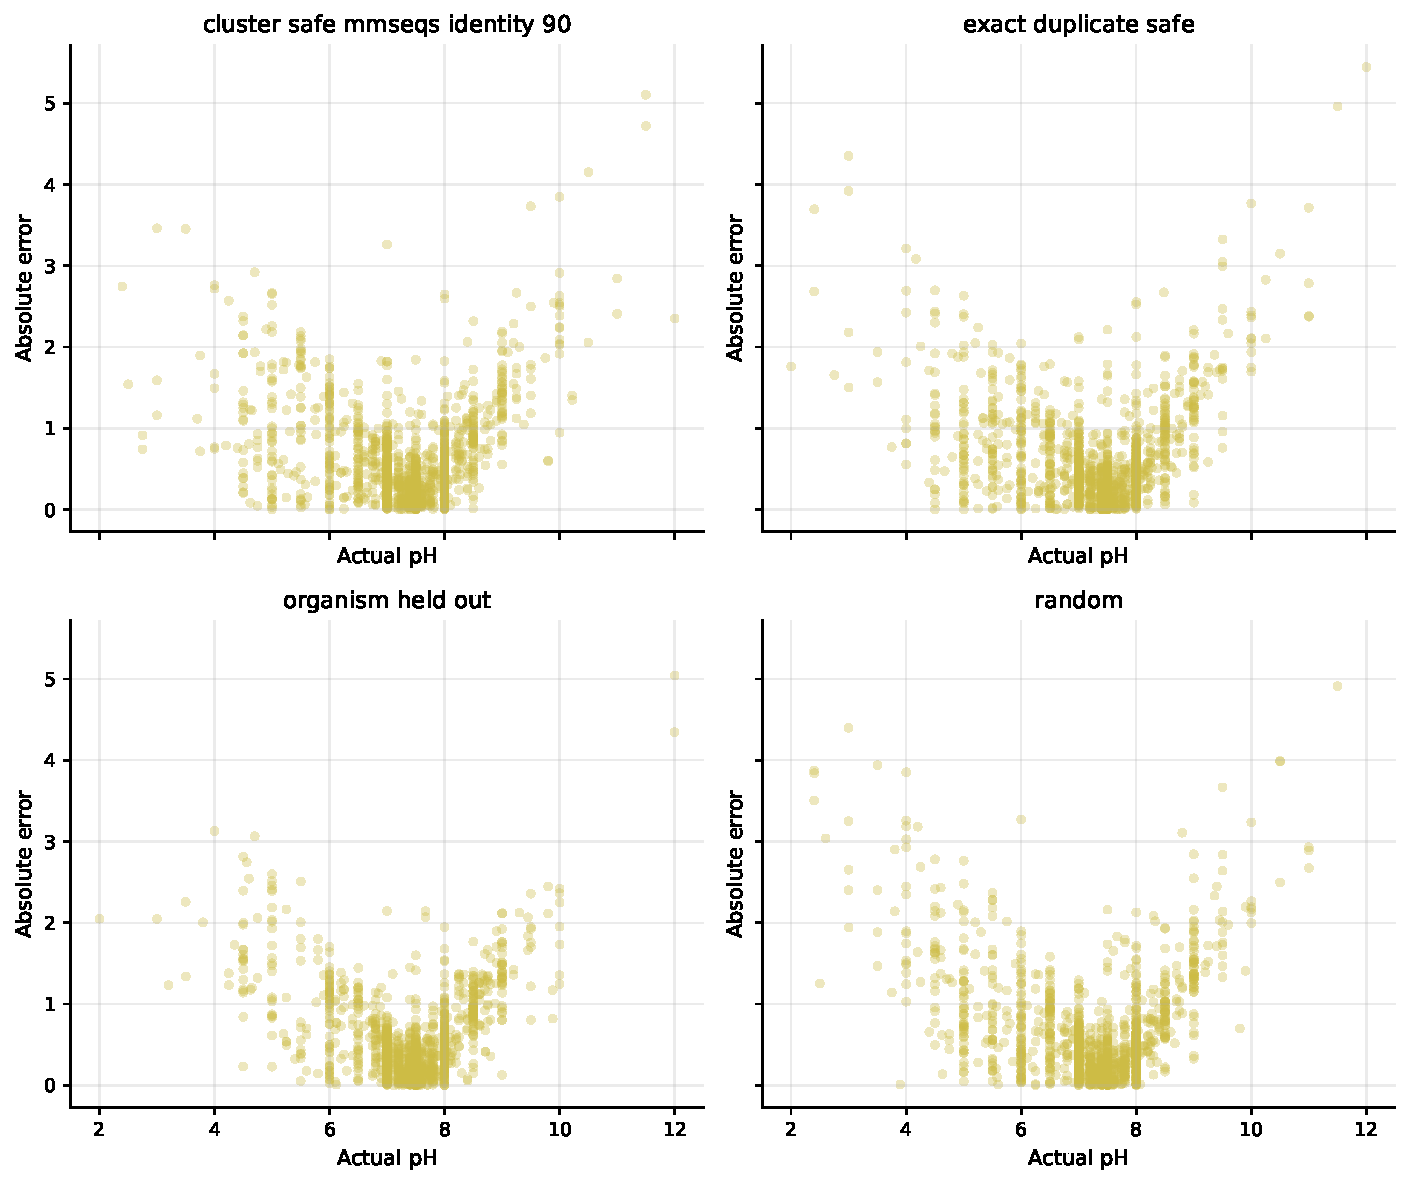
\includegraphics[width=\textwidth]{figures/error_vs_true_ph_best_embedding_models.pdf}
    \caption{Absolute prediction error as a function of true optimal pH for the selected best ESM-2 embedding models. The figure shows the generated diagnostic subset; complete split-strategy results, including the 50\%, 70\%, and EC-held-out evaluations, are reported in the tables.}
    \label{fig:error-vs-true-ph}
\end{figure}

\begin{figure}[htbp]
    \centering
    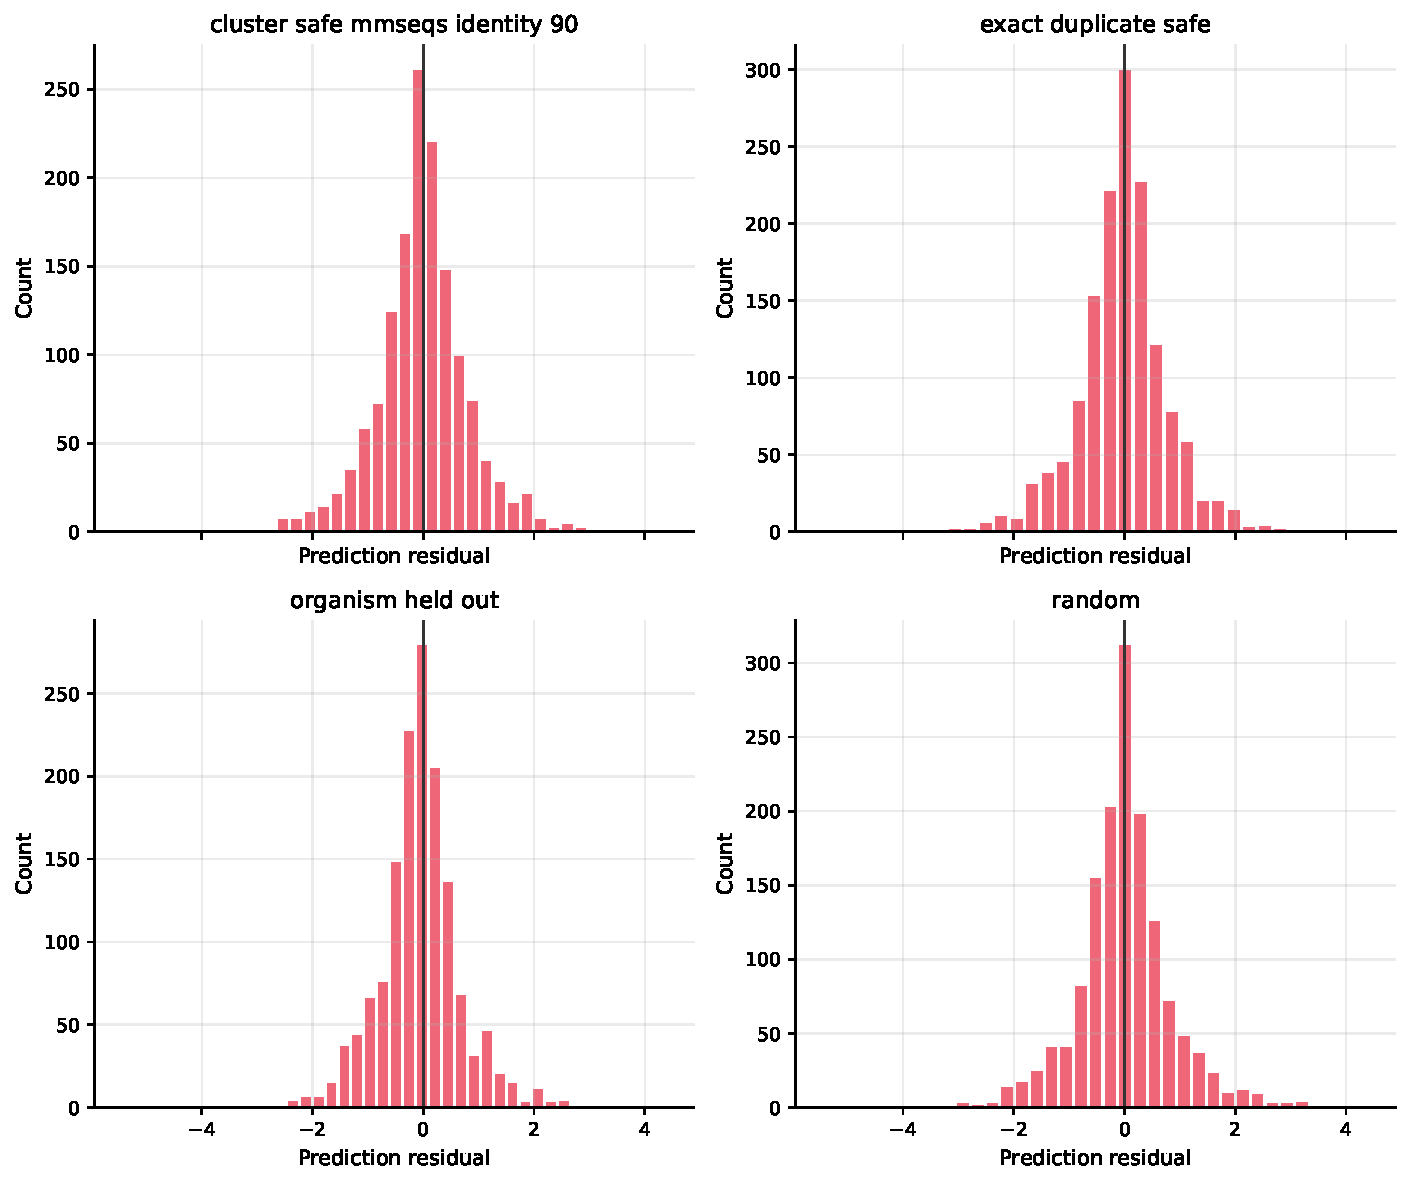
\includegraphics[width=\textwidth]{figures/residual_distribution_best_embedding_models.pdf}
    \caption{Residual distributions for the selected best ESM-2 embedding models. The figure shows the generated diagnostic subset; complete split-strategy results, including the 50\%, 70\%, and EC-held-out evaluations, are reported in the tables.}
    \label{fig:residual-distributions}
\end{figure}

Performance stratified by pH range is reported in Table~\ref{tab:performance-by-ph-range}; acidic, near-neutral, and alkaline are defined as pH $<6$, $6\leq\mathrm{pH}\leq8$, and pH $>8$, respectively. Additional error-analysis tables were exported to the supplementary output directory rather than placed in the main text.

\begin{figure}[htbp]
    \centering
    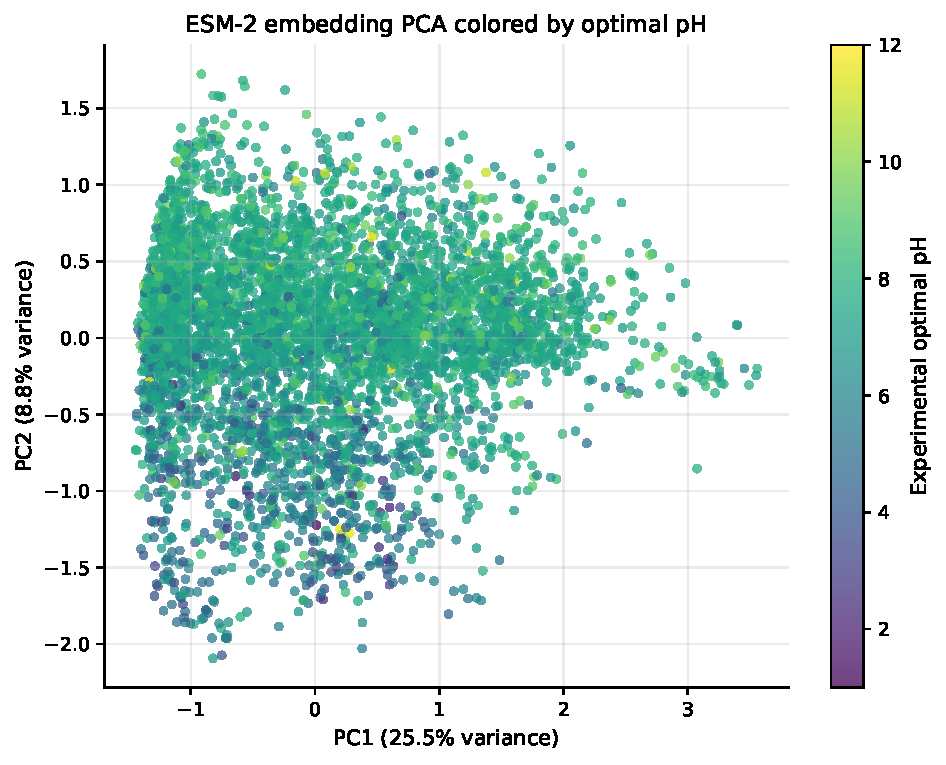
\includegraphics[width=0.78\textwidth]{figures/embedding_pca_optimal_ph.pdf}
    \caption{Principal-component projection of frozen ESM-2 embeddings colored by experimental optimal pH. This visualization is exploratory and does not imply that individual embedding dimensions correspond to biological mechanisms.}
    \label{fig:embedding-pca}
\end{figure}

\begin{figure}[htbp]
    \centering
    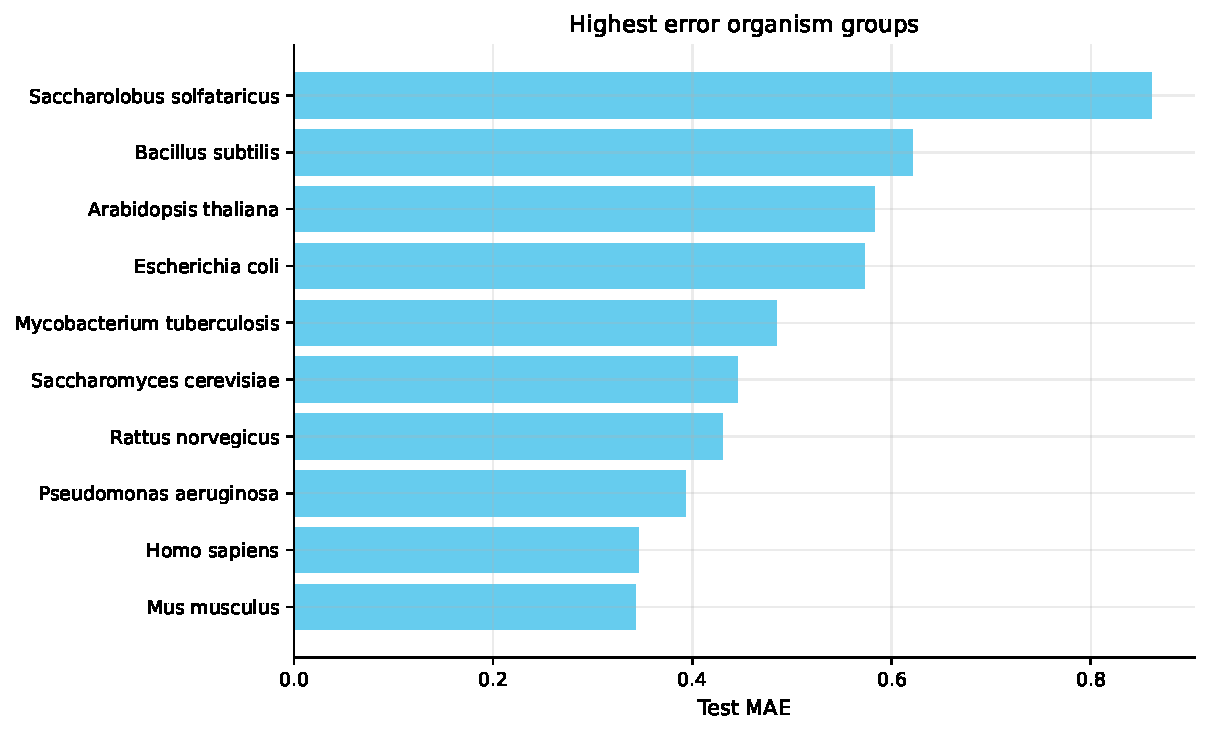
\includegraphics[width=\textwidth]{figures/error_by_organism.pdf}
    \caption{Highest-error organism groups among sufficiently represented test examples for the selected embedding-based model.}
    \label{fig:error-by-organism}
\end{figure}
